\section{Flutter}

\textit{Flutter} ist ein von \textbf{Google} entwickeltes \textit{User-Interface-Framework} zur
Entwicklung plattformunabhängiger Apps sowohl für Web, Desktop als auch Mobile.

Neben der Möglichkeit Apps für verschiedene Systeme erstellen zu können, ohne etwas mehrfach programmieren
zu müssen, bietet Flutter auch einen integrierten Widget-Katalog voll vorgefertigter UI-Elemente.\\
Diese können nach Belieben verwendet, umgestaltet und miteinander kombiniert werden.

Flutter bietet hiermit auch Personen mit weniger Erfahrung auf dem Gebiet der Softwareentwicklung
die Möglichkeit, relativ einfach eigene Apps zu entwickeln.

\subsection{Was macht Flutter besonders?}

\subsubsection{Design-Architektur}

Der Clou hinter Flutter steckt in seiner Architektur und Design-Struktur, denn in diesem Framework ist \textbf{alles} ein Widget,
von der eigentlichen App bis hin zum einfachen Text.

\begin{figure}[H]
    \begin{center}
        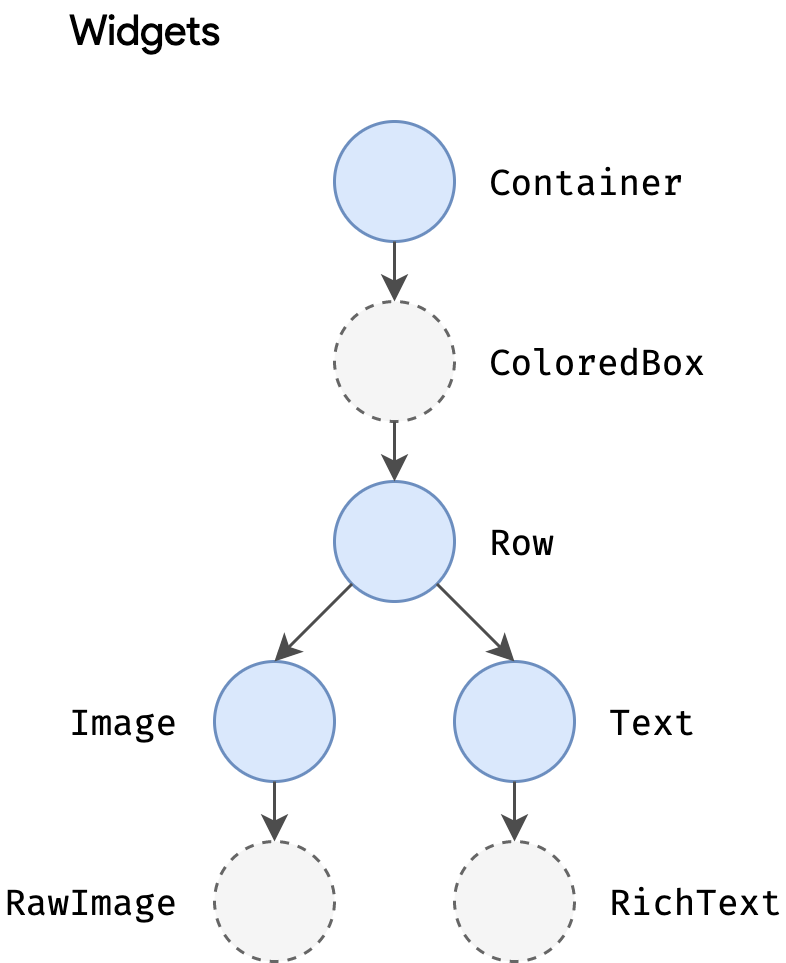
\includegraphics[width=0.5\textwidth]{images/Flutter/design-structure.png}
        \caption{Design-Struktur und Widget-Aufbau von Flutter}
        \cite{flutterDesignArchitecture}
        % https://flutter.dev/docs/resources/architectural-overview
    \end{center}
\end{figure}

Der Aufbau und das Erstellen eines User-Interfaces mithilfe von Flutter erfolgt in erster Linie
durch das Kombinieren, Zusammenbauen und Verschachteln von Widgets.
Abhängig von ihrem Zustand (\textit{Widget-State}) und ihren Attributen beschreiben jene Widgets, wie das entsprechende
View zur Laufzeit aussehen wird.

Ändert sich der Zustand eines Widgets, wird es erneut aufgebaut und gerendert. Die Flutter-Engine 
vergleicht dabei vorherige Zustände mit der neuen Änderung und rendert nur jene Widgets neu, die
sich auch wirklich verändert haben.

Auf diesem Wege kann der Renderprozess von Widgets so schnell wie möglich durchlaufen werden, wodurch auch die Performance der App gesteigert wird.

Auf diesem Prinzip baut auch Flutters \textit{Hot-Reload}-Funktion bei der Entwicklung auf. Mithilfe dieser
können Veränderungen an der App in wenigen Augenblicken auf den Emulator übertragen werden, ohne, dass es einen
Neustart der App bedingt.

So können selbst die kleinsten Veränderungen schnell ausprobiert und getestet werden, ohne einen erneuten Build von Grund auf
zu benötigen.

\subsubsection{Plattformunabhängigkeit}

Mithlfe von Flutter können Apps unabhängig von einer Zielplattform entwickelt werden. Das heißt, dass eine Codebase
sowohl als Android-App und iOS-App als auch als Web-App deployed werden kann.

Neben den enormen Zeitersparnissen werden ebenso die nötigen Kenntnisse zweier Programmiersprachen, beispielsweise
\textit{Kotlin} für Android und \textit{Swift} für iOS, auf \textbf{Dart} reduziert.

Unter anderem wird dies durch den oben erwähnten Widget-Katalog erzielt. Dieser bietet zwei Varianten
von Widgets an, einerseits die \textit{Material Components} für Android, andererseits die \textit{Cupertino Components}
für iOS.

Das jeweilige Widget-Paket passt sich adaptiv an das Design des entsprechenden Betriebssystems an, um einen möglichst
geringen UI-Kontrast zwischen App und dem Rest des Betriebssystems zu garantieren.

% Kombination von Material & Cupertino oder Default mit Custom Scrolls.

\begin{figure}[H]
    \begin{center}
        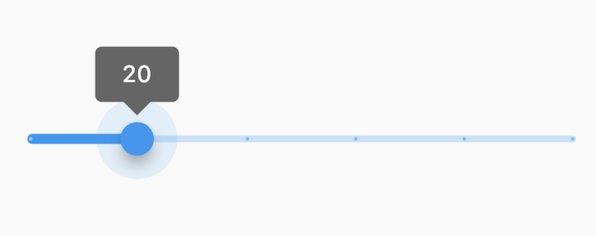
\includegraphics[width=0.5\textwidth]{images/Flutter/material-slider.png}
        \caption{Slider-Widget im Material-Design für Android}
        \cite{flutterMaterialSlider}
        % https://flutter.github.io/assets-for-api-docs/assets/material/slider.png
    \end{center}
\end{figure}

\begin{figure}[H]
    \begin{center}
        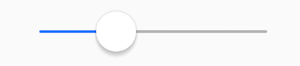
\includegraphics[width=0.5\textwidth]{images/Flutter/cupertino-slider.png}
        \caption{Slider-Widget im Cupertino-Design für iOS}
        \cite{flutterCupertinoSlider}
        % https://flutter.dev/images/widget-catalog/cupertino-slider.png
    \end{center}
\end{figure}

\subsection{Layoutting in Flutter}

Den Kern von Flutters Layout-System bilden, wie bereits erwähnt, die einzelnen Widgets, deren Attribute und ihr
kaskadierendes Verhalten zueinander.

\begin{figure}[H]
    \begin{center}
        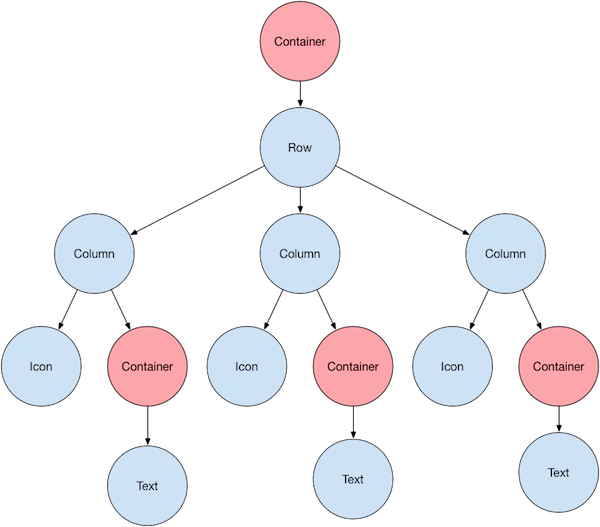
\includegraphics[width=0.65\textwidth]{images/Flutter/widget-tree.png}
        \caption{Widget-Tree für ein beispielhaftes Layout}
        % https://flutter.dev/images/widget-catalog/cupertino-slider.png
        \cite{flutterWidgetTree}
    \end{center}
\end{figure}

Ähnlich zu anderen Frameworks wie beispielsweise \textit{Bootstrap 4} können unter Einsatz von bekannten Standard-Widgets wie Containern, Rows und Columns bereits simple Layouts erstellt werden.

\newpage

Ein Widget wird in Flutter mithilfe des entsprechenden Objekt-Konstruktors an der gewünschten Stelle erzeugt und mit entsprechenden Attributen befüllt.

\begin{code}
    \centering
    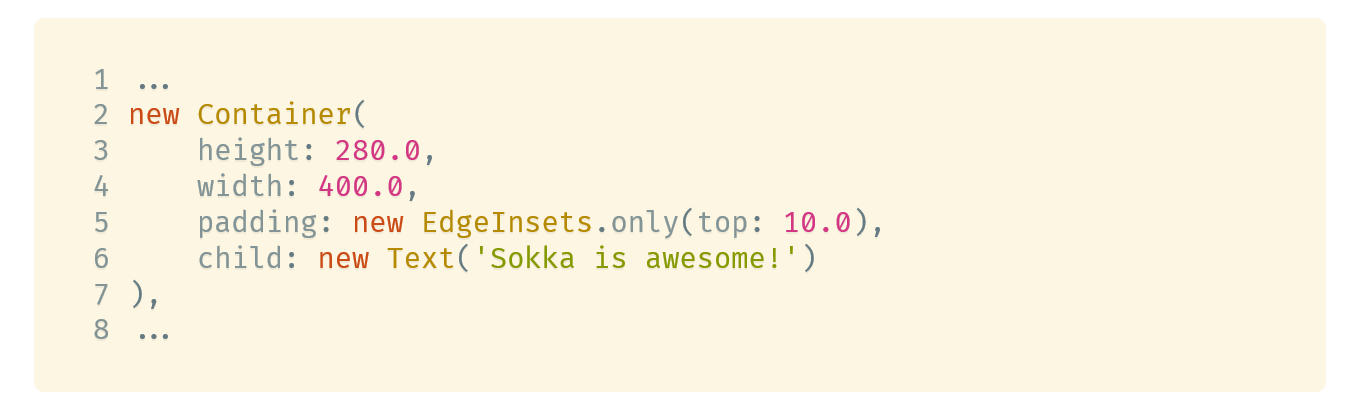
\includegraphics[width=1\textwidth]{images/Flutter/flutterCreateContainer.png}
    \caption{Erzeugen eines einfachen Container-Widgets mithilfe von Flutter}
\end{code}

Hiermit wird ein neues Container-Widget mit 280 Pixeln Höhe,
400 Pixeln Breite, einem Top-Padding von zehn Pixeln und einem Text als Kind-Widget erzeugt.

Wie bereits erwähnt können durch das Kaskadieren unterschiedlicher Widgets relativ einfach komplexe UI-Strukturen erzeugt werden. Hierfür müssen lediglich die weiteren / inneren Widgets dem \lstinline{child}- bzw. \lstinline{children}-Property des äußeren Widgets übergeben werden.

\begin{code}
    \centering
    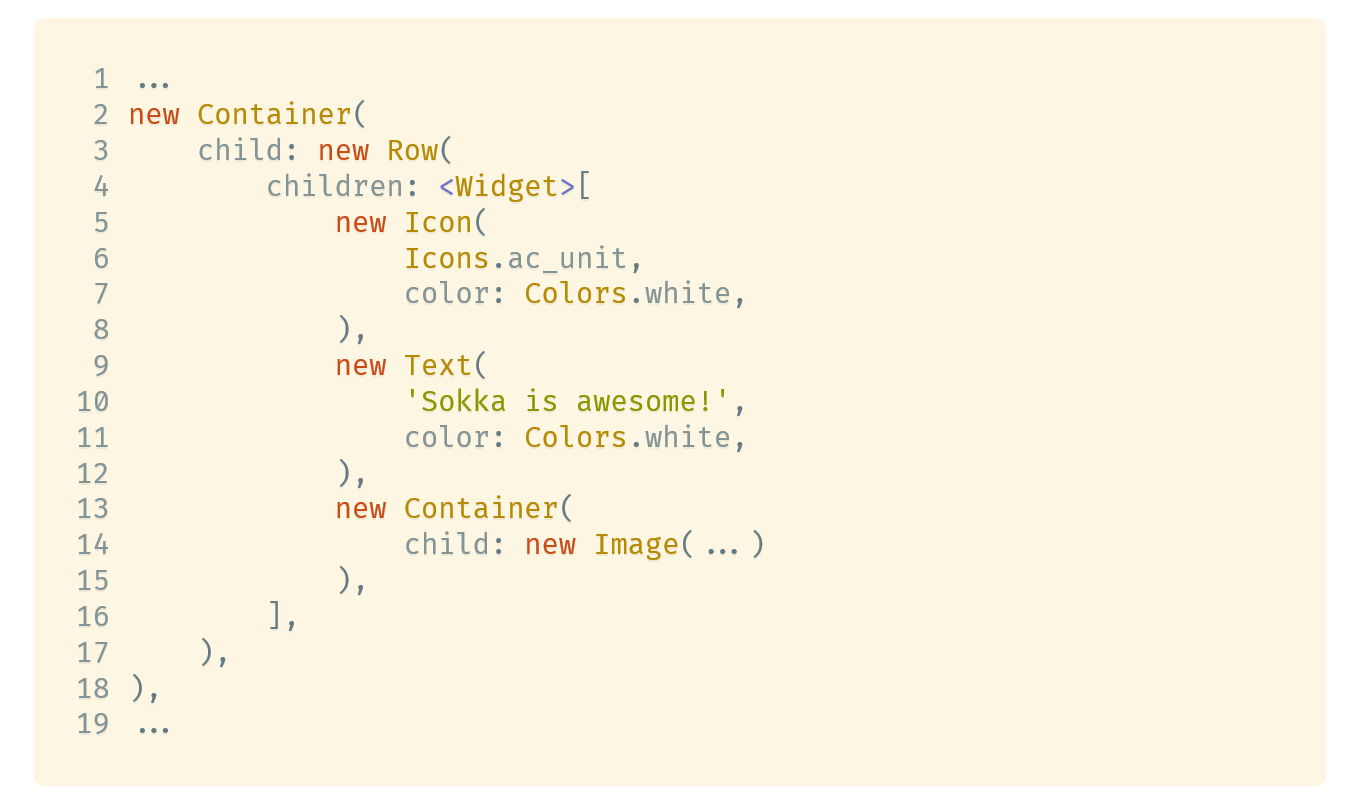
\includegraphics[width=1\textwidth]{images/Flutter/flutterCreateCascadingContainer.png}
    \caption{Erzeugen eines Containers mit verschachtelten Child-Widgets}
\end{code}

% https://flutter.dev/docs/development/ui/layout

\subsection{Rendern von Widgets}

Grundsätzlich erfolgt das Rendern eines Widgets über seine eigene \lstinline{build()}-Funktion. Diese wird aufgerufen,
sobald ein Widget gerendert bzw. neugerendert werden muss und retourniert ein entsprechendes Widget-Objekt,
der dem Design-Tree des entsprechenden Kontexts hinzugefügt wird.

\begin{code}
    \centering
    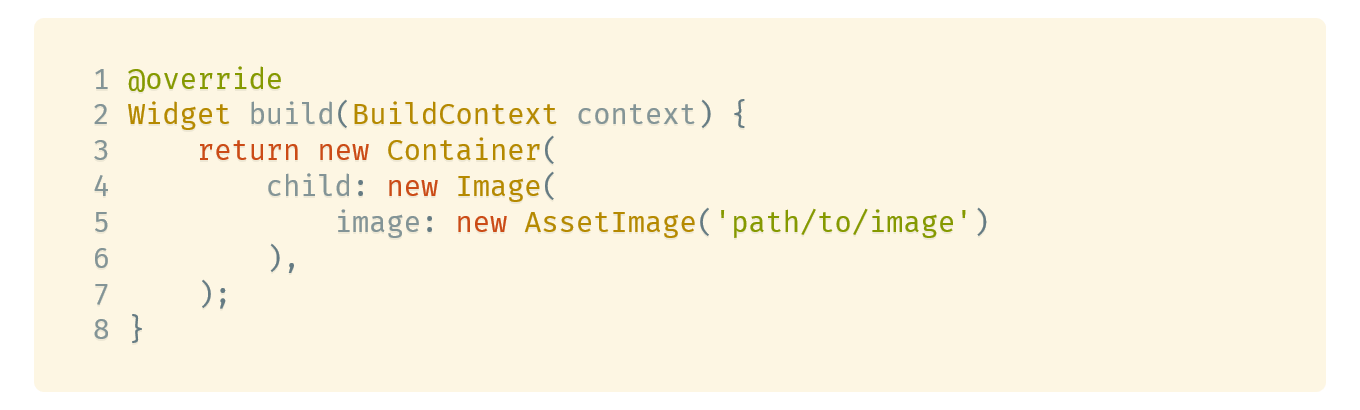
\includegraphics[width=1\textwidth]{images/Flutter/flutterBuildFunction.png}
    \caption{\lstinline{build()}-Funktion eines Widgets}
\end{code}

Obige Build-Funktion erzeugt einen neuen Container mit einem Bild als Child-Element und übergibt dieses
an den Widget-Tree des entsprechenden Layouts.

Hierbei gilt allerdings, zwischen zwei Arten von Widgets zu unterscheiden, den sogenannten \textit{Stateless Widgets}
und \textit{Stateful Widgets}.

Wie der Name bereits verrät, haben Stateless-Widgets einen definierten, statischen Zustand und reagieren nicht
auf das Verhalten anderer Widgets oder die Interaktion eines Nutzers, beispielsweise Icons, Text oder einfache
Buttons.

\begin{code}
    \centering
    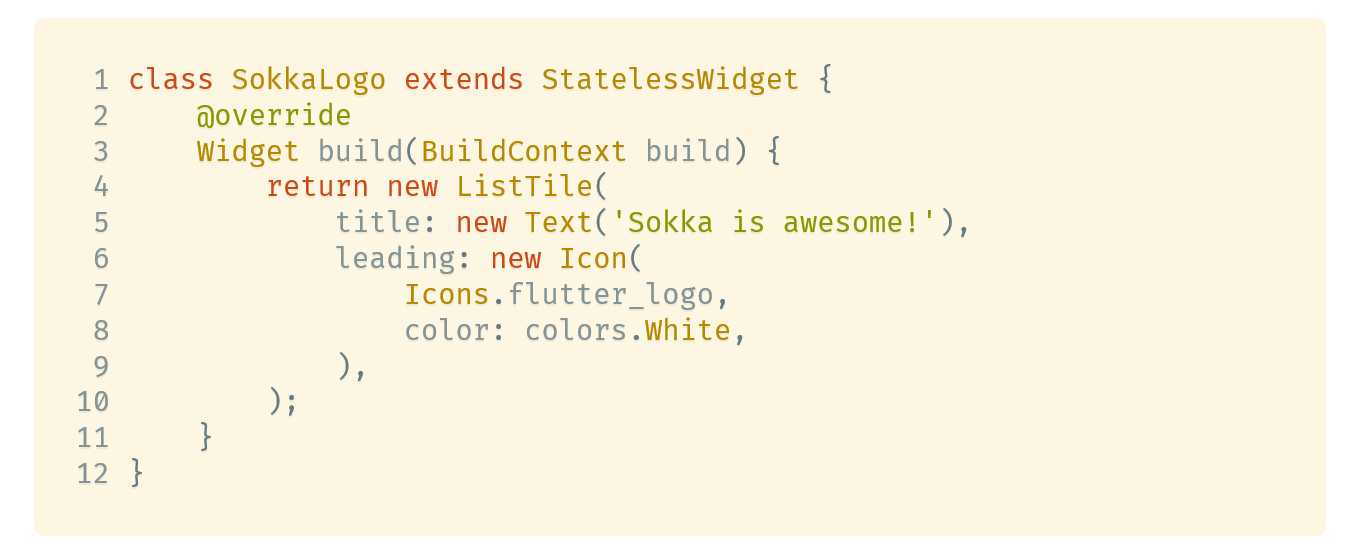
\includegraphics[width=1\textwidth]{images/Flutter/flutterStatelessWidget.png}
    \caption{Einfaches Stateless Widget}
\end{code}

Stateful-Widgets dagegen haben einen internen Zustand, welcher durch Interaktion mit dem Nutzer dynamisch verändert
werden kann, beispielsweise durch das Tippverhalten des Nutzers.

\subsection{Interaktivität der App}

% https://flutter.dev/docs/development/ui/interactive

Um für Interaktion der App zu sorgen werden, wie eben erwähnt, sogenannte Stateful-Widgets benötigt. Diese Widgets sind dynamisch und können beispielsweise ihr Aussehen als Reaktion auf Events, Input durch den Nutzer oder den Erhalt von Daten von einer API verändern.

Damit ein solches Widget weiß welchen Zustand es zum aktuellen Zeitpunkt hat, wird dieser in einem \textit{State}-Objekt vom Typ
des Widgets gespeichert. Ein solches State-Objekt besteht aus Werten, die den Zustand des entsprechenden Widget beschreiben können, beispielsweise ob ein ExpansionPanel (aufklappbare Karte) auf- oder zugeklappt ist oder der welchen Wert ein Slider-Widget aktuell hat.

Um den Zustand eines Widgets während der Laufzeit zu verändern und jene Änderung im Anschluss anzeigen zu können, wird hierfür die \lstinline{setState()}-Funktion verwendet.

Diese überschreibt die entsprechende Variable mit dem neuen Zustandswert und lässt die Flutter-Engine das entsprechende
Widget neu rendern, um die Veränderung direkt erkennbar zu machen.

\begin{code}
    \centering
    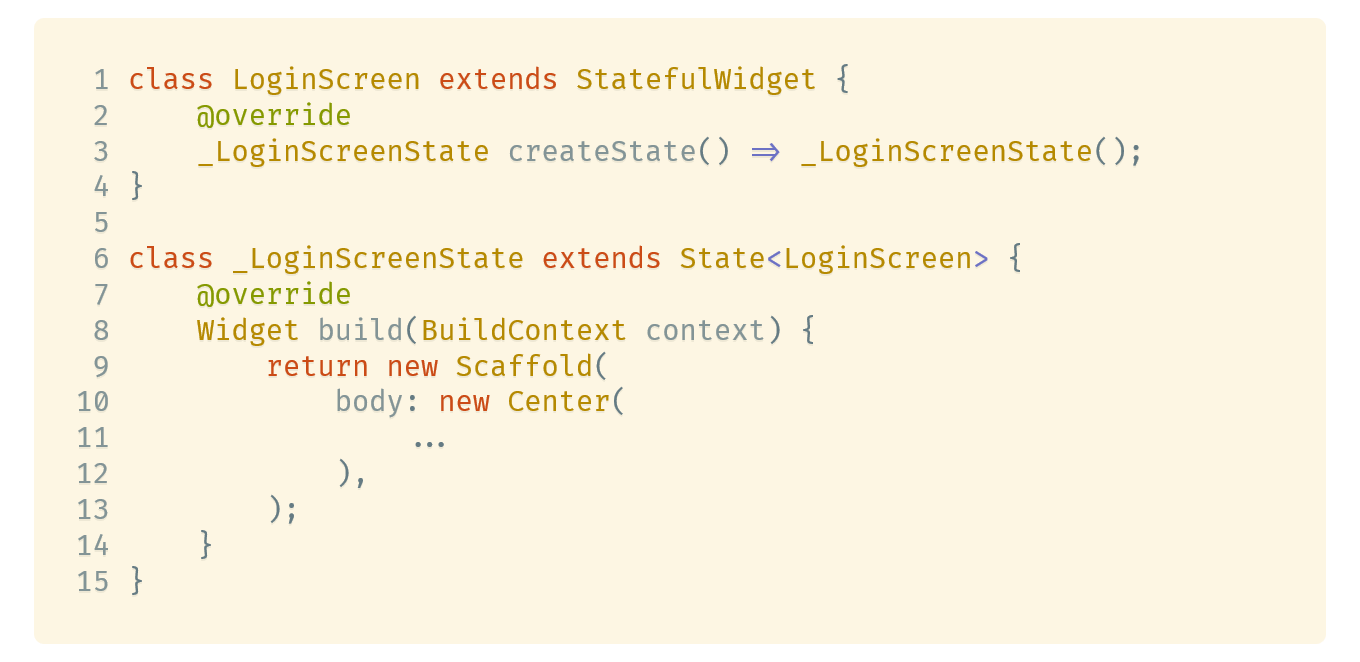
\includegraphics[width=1\textwidth]{images/Flutter/flutterStatefulWidget.png}
    \caption{Ein einfaches Stateful Widget}
\end{code}

Wie anhand der Implementation zu erkennen ist, ruft das Widget \textit{LoginScreen} die Build-Funktion
seines Zustandwrappers \textit{\_LoginScreenState} auf und erzeugt damit ein neues Widget mit dem entsprechenden
Zustand.

Ändert sich jener Zustand, so wird die Build-Funktion erneut mit einem anderen Zustand aufgerufen und das Widget wird neu gerendert.

\subsubsection{App-States und ephemerale States}

% https://flutter.dev/docs/development/data-and-backend/state-mgmt/ephemeral-vs-app

In Bezug auf die Widget-Architektur von Flutter gilt es zwei Arten von Zuständen zu unterscheiden:

\paragraph{Ephemerale States}

Unter sogenannten ephemeralen Zuständen, auch UI-Zustände oder lokale Zustände genannt, versteht man Zustände, welche in
einem einzelnen Widget gespeichert werden können. Ein ephemeraler Zustand ist also vergleichbar mit einer veränderbaren, lokalen Variable einer Klasse oder eines Scopes.

Einfache Beispiele hierfür sind etwa
\begin{itemize}
    \item der Fortschritt eines Animationsprozesses
    \item aktuell ausgewählter Tab in einer BottomNavigationBar
    \item die aktuelle Zahl an Widgets in einem ListView
\end{itemize}

\paragraph{App-States}

Im Gegensatz zu ephemeralen Zuständen werden App-Zustände global über die gesamte App gespeichert und können daher an jedem Ort in der App abgerufen und verändert werden.

Beispiele im konkreten Fall von Sokka sind unter anderem
\begin{itemize}
    \item E-Mail-Adresse und Session-Token der aktuellen Usersitzung
    \item Aktuell verfügbare Menüs und Produkte
    \item Gespeicherte Menüs und Produkte im Warenkorb
    \item alle Bestellungen des angemeldeten Nutzers
\end{itemize}

\subsection{Navigation und Routing durch die App}

Um zwischen den verschiedenen Screens und Views der App zu wechseln und zu navigieren benötigen wir die \textit{Navigator}-Klasse von Flutter.

Hierfür ist es sinnvoll zuerst eine \textit{HashMap} mit allen möglichen Routes der App zu definieren
um so benannte Routen (\textit{named routes}) verwenden zu können.

\begin{code}
    \centering
    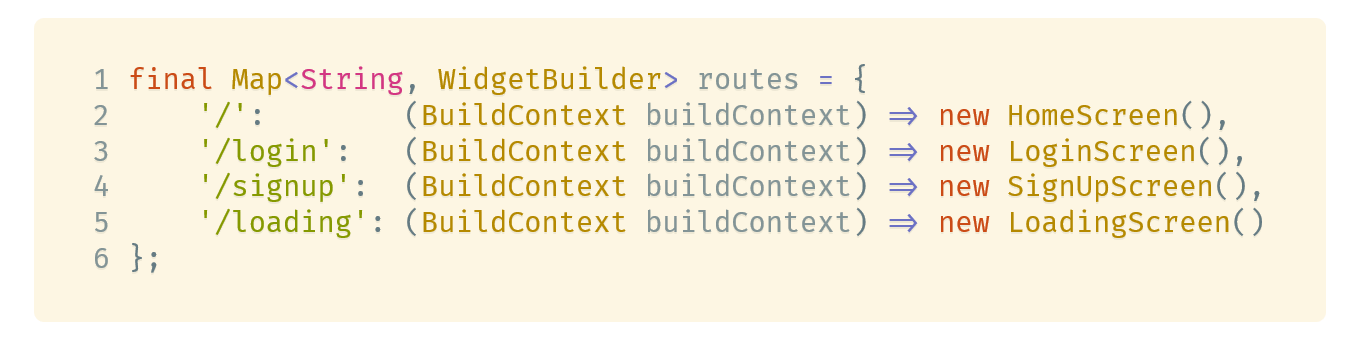
\includegraphics[width=1\textwidth]{images/Flutter/flutterRoutes.png}
    \caption{Routes für die Navigation zwischen Screens}
\end{code}

\newpage

Diese Routes müssen im Anschluss dem \textit{routes}-Property des MaterialApp-Widgets unserer App übergeben werden.

\begin{code}
    \centering
    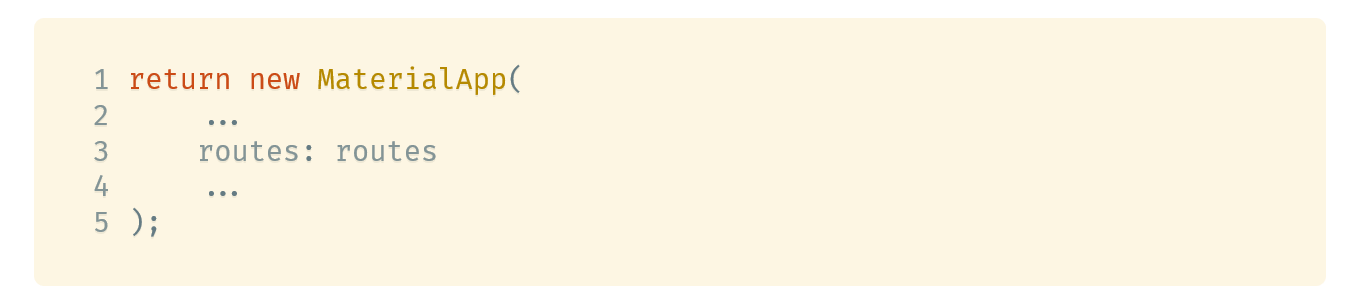
\includegraphics[width=1\textwidth]{images/Flutter/flutterMainRoute.png}
    \caption{Setzten der Routes im App Entry-Point}
\end{code}

Nun kann mithilfe der Navigator-Klasse und unseren definierten Routes einfach durch die App navigiert werden.

Hierfür stehen einige Methoden zur Verfügung:

\begin{code}
    \centering
    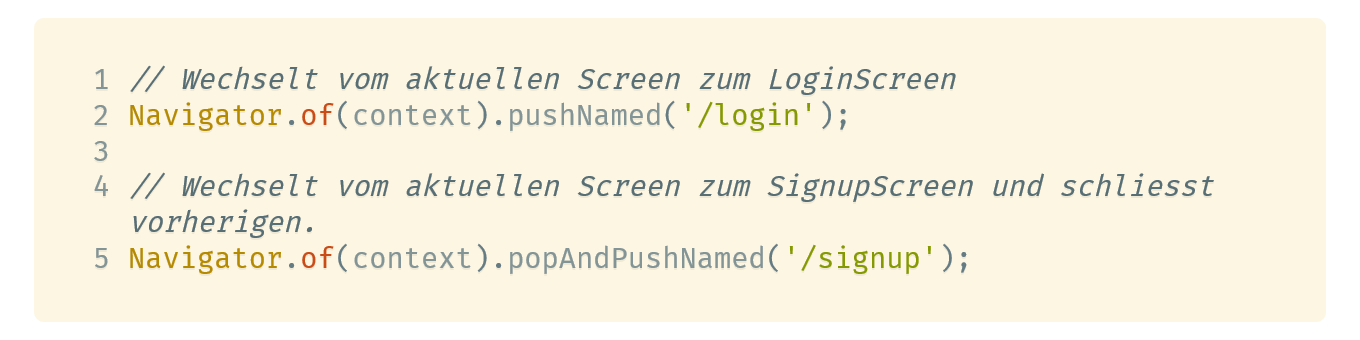
\includegraphics[width=1\textwidth]{images/Flutter/flutterNavigatorOf.png}
    \caption{\lstinline{Navigator.of()}-Funktion zum Wechseln der Screens per \textit{namedRoutes}}
\end{code}

Alternativ kann auch ohne NamedRoutes durch die App mithilfe der (umständlicheren) \lstinline{push()}-Funktion navigiert 
werden.

\begin{code}
    \centering
    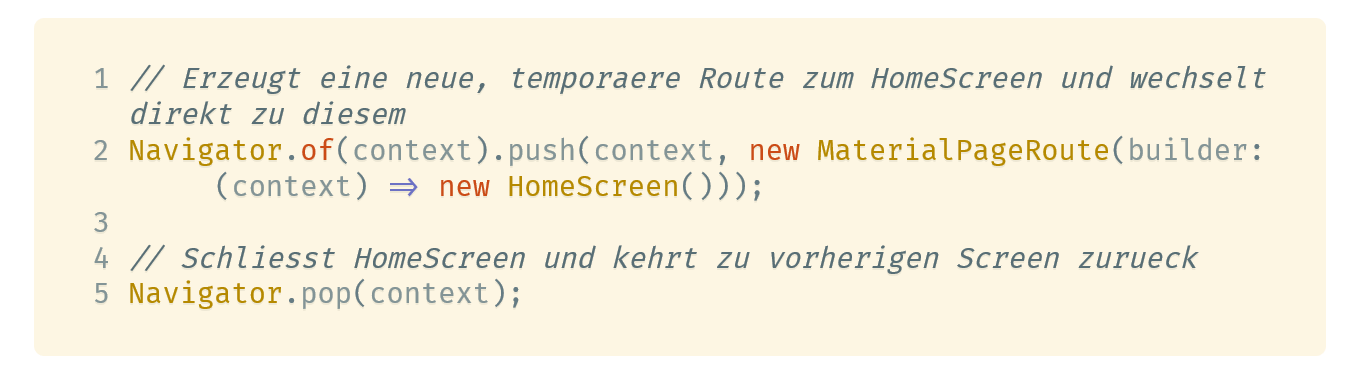
\includegraphics[width=1\textwidth]{images/Flutter/flutterAlternateNavigator.png}
    \caption{Navigieren durch die App per MaterialPageRoutes}
\end{code}